\section{Introduction}
This section will show step by step, how the source of a \languageName{} template, is compiled, and transformed into a \acro{HTML} file. In general compilers tend to follow the diagram shown in Figure~\ref{fig:compilerSteps}. However \languageName{} is going to be compiled down to \acro{HTML}, not machine code. So there is little/nothing to optimise about the code. Polly also has multiple Symbol Tables. One for holding variables, another for holding component definitions, and a final one for holding functions, that are defined from Rust. See Figure~\ref{fig:pollySteps}.

\begin{figure}[!htbp]
    \centerline{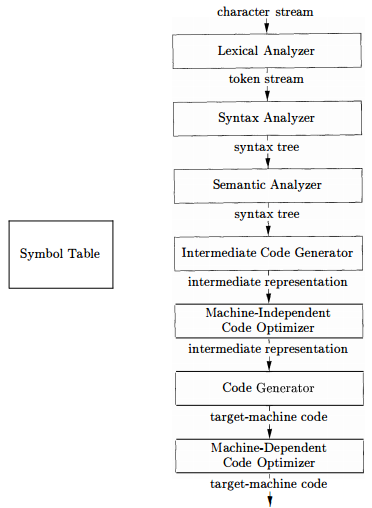
\includegraphics[width=0.7\textwidth]{img/compiler_steps.png}}
    \caption{Traditional steps of a compiler\cite{DragonBook}.}
    \label{fig:compilerSteps}
\end{figure}

\begin{figure}[!htbp]
    \centering
    \begin{tikzpicture}[squarednode/.style={rectangle, draw=black!60, fill=black!5, very thick, 
    minimum width=50mm, minimum height=10mm},]

    \node[](source){source program};
    
    \node[squarednode](lexer)[below=of source]{Lexer};

    \node[](lexemes)[below=of lexer]{Lexemes};
    
    \node[squarednode](parser)[below=of lexemes]{Parser};
    \node[](ast)[below=of parser]{\acro{AST}};

    \node[squarednode](codegen)[below=of ast]{Code Generation};
    
    \node[](html)[below=of codegen]{HTML};

    \node[squarednode](components)[left=of parser]{Component Symbol Table};
    \node[squarednode](variables)[above=of components]{Variable Symbol Table};
    \node[squarednode](functions)[below=of components]{Function Symbol Table};

    \draw[->] (source.south) -- (lexer.north);
    \draw(lexer.south) -- (lexemes.north); 
    \draw[->] (lexemes.south) -- (parser.north); 
    \draw (parser.south) -- (ast.north);
    \draw[->] (ast.south) -- (codegen.north);
    \draw[->] (codegen.south) -- (html.north);


    \end{tikzpicture}
    \caption{Polly's compiler steps \cite{DragonBook}.}
    \label{fig:pollySteps}
\end{figure}



\section{Compiling a template.}
In order to show how \languageName{} compiles a program. It is best shown through a example. The example program is shown in Figure~\ref{fig:sampleProgram}. It is a very simple \textit{``Hello World''} in \languageName{}. All the template is doing is placing a header on the page with ``World'' underlined. First thing that is needed to understand is that Figure~\ref{fig:sampleProgram} is what humans see, with characters hidden for legibility.

\subsection{Lexer}
Firstly the lexer divides each character of the source is then divided into a Iterator(An array of variable length) consisting of tuples(An ordered list of elements) consisting of the character and it's position in the source file.

The \compiler{} keeps track of the characters position in order to provide accurate error messages, showing exactly where the syntax is incorrect. The lexer iterates through the iterator using two functions. \textit{``next()''}, and \textit{``peek()''}. The function \textit{``next()''} takes the next element in the iterator, and advances it's position, so repeatedly calling the function \textit{``next()''} would advance through all the elements. \textit{``peek()''} takes the next element in the iterator, but doesn't advance it's position. So calling \textit{``peek()''}, and then \textit{``next()''} would return the same element.

\begin{figure}[!htbp]
    \begin{verbatim}
        /h1{Hello /u{World}!}
    \end{verbatim}
    \caption{The source of the example.}
    \label{fig:sampleProgram}
\end{figure}

\begin{figure}[!htbp]
    \begin{minted}{rust}
        [
            (0,  '/'), (1,  'h'), (2,  '1'), 
            (3,  '{'), (4,  'H'), (5,  'e'), 
            (6,  'l'), (7,  'l'), (8,  'o'),
            (9,  ' '), (10, '/'), (11, 'u'),
            (12, '{'), (13, 'W'), (14, 'o'),
            (15, 'r'), (16, 'l'), (17, 'd'),
            (18, '}'), (19, '!'), (20, '}')
        ]
    \end{minted}
    \caption{The array of tuples the lexer generates.}
    \label{fig:charIndices}
\end{figure}


The lexer then iterates through tuples, checking each character. If a character is a symbol which is defined in Figure~\ref{fig:lexemes}. It is then parsed into an abstract representation of it using a enum(Enumerated type) see Figure~\ref{fig:lexemes}. If the character is not any of the symbols, the \compiler stores it, and keeps parsing and concatenates all letters into a word.

All whitespace is ignored, and discarded by the lexer, except when there is space around a character, this is to preserve the format of the text. However the lexer will only store one leading, or following space, so \textit{``Hello··World!''} is concatenated to \textit{``Hello·World!''} Both are defined using the \textit{``Lexeme''} enum, which stores the position of the element from the file. See Figure~\ref{fig:lexerOutput} for the output of the Lexer. The lexer's only job is to separate the operators from the words, and provide a slightly more abstract representation of the source file. It doesn't define any logic, or hierarchy.

\begin{figure}
    \begin{minted}{rust}
        pub enum Lexeme {
            Symbol(usize, Operator),
            Word(usize, String),
        }

        pub enum Operator {
            /// The & character used for defining components.
            Ampersand,
            /// The @ character used for defining variables.
            At,
            /// The \ character used for escaping characters.
            BackSlash,
            /// The } character used to singify the end of an 
            /// element.
            CloseBrace,
            /// The ) character used to define the end of a
            /// function call, or attributes list.
            CloseParam,
            /// The , character used to separate arguments 
            /// within a component or function.
            Comma,
            /// The \$ sign used to define a function call.
            Dollar,
            /// The . character used for defining CSS classes
            /// attached to an element.
            Dot,
    \end{minted}
            continued on Figure~\ref{fig:lexemes2}
    \caption{Lexemes for \languageName{}}
    \label{fig:lexemes}
\end{figure}

\begin{figure}
    \begin{minted}{rust}
            /// The = character used for assignment within the
            /// attributes field
            Equals,
            /// The / character used to define elements
            ForwardSlash,
            /// The { character used to signify the start of 
            /// an elements children.
            OpenBrace,
            /// The ( character used to signify the start of 
            /// the attributes for an element, or start of a 
            /// function call
            OpenParam,
            /// The # character used to define CSS ids for an 
            /// element.
            Pound,
            /// The " character used for values within an 
            /// attributes field.
            Quote,
        }
    \end{minted}
    \caption{Lexemes for \languageName{}. Pt.2}
    \label{fig:lexemes2}
\end{figure}

\begin{figure}[!htbp]
    \begin{minted}{rust}
        [
            Symbol(0, ForwardSlash),
            Word(1, "h1"),
            Symbol(2, OpenBrace),
            Word(3, " Hello "),
            Symbol(8, ForwardSlash),
            Word(9, "u"),
            Symbol(10, OpenBrace),
            Word(11, "World"),
            Symbol(16, CloseBrace),
            Word(17, "!"),
            Symbol(18, CloseBrace)
        ]
    \end{minted}
    \caption{Lexer Output.}
    \label{fig:lexerOutput}
\end{figure}



\subsection{Parser}

\subsubsection{Introduction}
The parser takes the output of the lexer, and generates an \acro{AST}. This is where the bulk of the work is done, in terms of determining how the logic is structured, and what the syntax means. The parser has two main contexts, the top level, and the context after certain symbols are defined. The main reason for this is to allow certain operators to have meaning in without requiring \you{} to have to ``escape'' the operators every time they were used. One prime example of this is the \textit{``.''}, or \textit{``Dot''} symbol.

It is used a lot of contexts from being used for \acro{CSS} selectors, and name-spaced identifiers, but if \you{} were writing a paragraph it would be very cumbersome to have to ``escape'' every full stop in a paragraph. So having different contexts allows the syntax, both utilise the \textit{``.''}, for there paragraphs, but also use it with elements for \acro{CSS} class selectors, and to name space variables, and component names.

\begin{figure}[!htbp]
    \begin{minted}{rust}
        pub enum Token {
            Html(Element),
            Text(String),
            Variable(String),
            CompCall(ComponentCall),
            Function(FunctionCall),
        }
    \end{minted}
    \caption{The token enum for the parser.}
    \label{fig:tokenEnum}
\end{figure}

\subsubsection{Text.}
Under the main context, the compiler first checks which lexeme was given. If the lexeme is a \textit{``Word''}, the compiler stores it, and checks if the next lexeme is also a \textit{``Word''}, if it is the compiler then adds it to the previous \textit{``Word''}. The compiler repeats this until the next lexeme isn't a \textit{``Word''}, creating a \textit{``Text''} node, that represents a paragraph.

\textit{``Text''} is a terminal node, meaning that it cannot have any child nodes. Since \textit{``Text''} is purely text, and there is no further logic that can be applied, the positions of each of the words is discarded.

\subsubsection{Variables.}
The next check is to see if the lexeme is a \textit{``@''}, or \textit{``At''} symbol. The \textit{``At''} symbol defines a variable, and the name should map to \acro{JSON} object that is passed to the template. The compiler then takes the next name-spaced identifier.

Where a name-spaced identifier is a a series of lexemes starting with a \textit{``Word''}, and any amount of words providing the previous word was following by a   \textit{``Dot''} symbol e.g. \textit{``@john.doe''}. The \textit{``Variable''} node is also a terminal node. If the next symbol isn't a \textit{``Word''}, the parser will instead provide an error.

\subsubsection{Elements.}
The proceeding check is if the lexeme is a \textit{``/''}, or \textit{``ForwardSlash''} symbol. This is one of the most complex sections of the parser, as during the element definition context, as nearly every symbol has a different meaning. When parsing the element's definition, the compiler takes the first \textit{``Word''}, and defines that as the element's tag, or name e.g. \textit{h1, p, div}. 
\newpage
This identifier cannot be name-spaced, like other nodes, as the  \textit{``Dot''} symbol is used to define a class in the element definition context, and providing it so that at the start of an element's definition, the \textit{``Dot''} symbol has a different use would be unintuitive. 

Within the element definition context, the compiler then checks for the presence of an \textit{``\&''}, or \textit{``Ampersand''} symbol. This defines that instead of having a static body content, the element will instead call this component, optionally with any arguments passed in. The result of the component call, will instead become the body of the element. This means that the element can't also have a static body of text, as it would be confusing for \you{} on where the body of the text would go in the element in relation to the component call's body. This is type of Component call is called a resource.

Since both classes, and id's are the most used html attributes they are given special syntactic sugar in the form of being able to attach CSS selectors. These both take a similar form as the element definition with a \textit{``Dot''} symbol, or \textit{``\#''} or \textit{``Pound''} symbol. Then having the next symbol taken as the name of the class, or id. If it is a \textit{``Word''}, then it is added to the element as a class, or id, if it isn't an error is provided.
Since element attributes are arbitrary, and can take numerous forms, \you{} can also a attach a pair of \textit{``()''}, or \textit{``OpenParam''}, and \textit{``CloseParam''} symbols. Inside these parameter blocks \you{} can define any type of attribute from the traditional key, value pairing e.g. \textit{action=``POST''}, to single word attributes e.g. \textit{``required''}.

All previous symbols can happen in any order after the element definition, so you can have  Class, Id, Class, Resource, Attributes, or Attributes, Resource, Id, Class, Class. To signify the end of defining an element, an \textit{``\{''}, or \textit{``OpenBrace''} symbol. This defines the body of the element. The compiler ignores all lexemes until it finds the appropriate \textit{``\}''}, or \textit{``CloseBrace''}. To do nesting the compiler starts a variable named \textit{``depth''} which starts at zero.
\newpage
As the compiler collects the lexemes, it check if it encounters a \textit{``OpenBrace''}, or \textit{``CloseBrace''}. If the compiler collects a \textit{``OpenBrace''} \textit{``depth''} is incremented by one. If it finds a \textit{``CloseBrace''} \textit{``depth''} is decremented by one. This continues  infinitely until it encounters a \textit{``CloseBrace''}, while \textit{``depth''} is zero. The parser then creates another child parser, and passes the collection of lexemes taken, and attaches the result of this parser to the element.

Additionally, as a form of syntactic sugar if the element ends with attributes, then the braces aren't required for the element. This was designed for \textit{``void''} element e.g. \textit{``meta, link, img''}, but can work for any element.

\subsubsection{Escaping.}
Previously mentioned was how the compiler allows \you{} to be able to have main context symbols used for user facing text. The \textit{``\textbackslash''}, or \textit{``BackSlash''} operator will just convert, the next symbol in the iterator to it's text version, and return a new \textit{``Text''} node containing it.

\subsubsection{Components.}
A component is simply a reusable piece of \languageName{} code. It can also be passed in variables. It does this in a similar way to how it parses the attributes, but instead of key, value pairings. It is is the symbol, plus the name \you{} wants to give the parameter. This parameter is alias, and stored in the component, so \acro{JSON} passed to the parent template, won't poison the component, and provide it values that weren't intended. Components get children in the exact same way as elements.
\newpage
\subsubsection{Functions.}
Unlike Components, and Elements, Functions can't be defined in \languageName{}, so the parser doesn't need to parse the logic of the functions. A \languageName{} function in Rust, takes a reference counted pointer\footnote{A referenced counted pointer, is a data type which tracks the references to it, deallocating when the reference count is zero}, to a reference cell\footnote{A Reference Cell is a data type in Rust, allowing interior mutability, and moving borrow checking to runtime} to the parent template. \verb|Rc<RefCell<Template>>| Functions only take in named arguments, in order to have a cleaner function API in Rust. This works exactly like the attributes in elements.


\begin{figure}[!htbp]
    \centering
    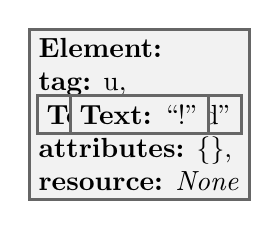
\begin{tikzpicture}[squarednode/.style={rectangle, draw=black!60, fill=black!5, very thick,},]
    \tikzset{level distance=120pt, sibling distance=72pt}
        \Tree[.\node[squarednode, align=left]{
                    \textbf{Element:}\\ 
                    \textbf{tag:} h1,\\
                    \textbf{classes:} [],\\ 
                    \textbf{attributes:} \{\},\\ 
                    \textbf{resource:} \textit{None}}; 
               [.\node[squarednode]{\textbf{Text:} ``Hello''}; ] 
               [.\node[squarednode, align=left]{
                    \textbf{Element:}\\ 
                    \textbf{tag:} u,\\
                    \textbf{classes:} [],\\ 
                    \textbf{attributes:} \{\},\\ 
                    \textbf{resource:} \textit{None}};
                    [.\node[squarednode]{\textbf{Text:} ``World''}; ] ]
               [.\node[squarednode]{\textbf{Text:} ``!''}; ]  ]
    \end{tikzpicture}
    \caption{The \acro{AST} of the example.}
\end{figure}

\subsection{Code Generation.}

Code generation is where the \acro{AST} is converted into the actual desired output, e.g. \acro{HTML}. While this project only focuses on HTML generation, there is no reason in the future the compiler could be expanded to generate other markup languages, such as \acro{XML}. 

Elements are generated first by allocating a String starting with a \textit{``<''}. The elements tag is then added \textit{``<h1''}. The Code generator then checks the elements other properties. If there are any classes they are added, same with attributes. Once that is done a \textit{``>''}, the code generator checks if the element has a resource, or has children, if it has a resource, the code generator calls the component, and creates a new code generator containing the resulting \acro{AST}, and takes that result, appends that to the string. The same is done for direct children, but with the component call Figure~\ref{fig:result}. Components, variables, and Functions are all generated the same way.

\begin{figure}[!htbp]
    \begin{minted}{html}
        <h1>Hello <u>World</u>!</h1>
    \end{minted}
    \caption{The end result.}
    \label{fig:result}
\end{figure}

\subsection{Template}
All of this is provided in a top level API call \textit{``Template''} which stores the functions, components, and \acro{JSON}. The template based on what language passed is passed into the render, will generate the components from the locales files.
\newpage
\section{An advanced example.}
The previous section demonstrated how the compiler works through an example. This section intends to show how the \you{} can actually take advantage of the process of \languageName{}'s compilation steps to perform much more complicated tasks, without compromising on your template by adding complex logic.

One of the most common use-cases for a templating language is to take an array of data that is of unknown length, and format the data into elements. For example a social media website might have a list of friends for a particular user. The website can't know how many every user is going to have, so it has to be designed around the possibility of infinite. See Figure~\ref{fig:websiteTemplate} for the template. It is a relatively simple template, with standard html, the only two new elements are a function call, and a component. The \textit{``std.each''} function takes two named arguments \textit{``array''} \& \textit{``component''}. \textit{``array''} represents the actual array of data to be used, and \textit{``component''} is the template to render for each entry of the array. The component which can simply be described as a reusable section of \acro{HTML}. This component also takes two arguments \textit{``@name''} \& \textit{``@picture''}.

\begin{figure}
    \begin{verbatim}
        /!DOCTYPE(html)
        /html {
            /body {
                /ul#friends-list {
                    $std.each(array = @friends, component = &friend)
                }
            }
        }

        &friend(@name, @picture) {
            /li {
                /img(src=@picture)
                /h4{@name}
            }
        }
    \end{verbatim}
    \caption{Friends list template using function, and components.}
    \label{fig:websiteTemplate}
\end{figure}

\begin{figure}[!htbp]
    \begin{minted}{json}
        {
            "friends": [
                {"name": "Jerry", "picture": "./imgs/jerry.png"},
                {"name": "Elaine", "picture": "./imgs/elaine.png"},
                {"name": "George", "picture": "./imgs/george.png"},
                {"name": "Cosmo", "picture": "./imgs/cosmo.png"}
            ]
        }
    \end{minted}
    \caption{Sample \acro{JSON}.}
    \label{fig:sampleFriends}
\end{figure}
One key steps that is applied to components is that once they are parsed, they are passed into a \textit{``Component Table''} as seen previously in Figure~\ref{fig:pollySteps}. Being placed in a separate table allows for the component to be used regardless of where it was declared as seen in Figure~\ref{fig:websiteTemplate} where the component is is passed to the function before it has been declared. This also allows for importing components, so \you{} can have separate files containing only components and use them in other files. 
\newpage
\subsection{Functions}
Functions behave a lot in the same way as components, but their difference is in the internal logic. Where a component can only generate a very predictable, and partially static html, functions can perform virtually any task as they are defined in Rust, and thusly have access to every library, and every capability Rust has. Functions have full knowledge of the \acro{JSON} that was passed meaning that a function can behave differently  based on types, for example if it was passed an array than if it was passed an object. Functions also have complete access to the component's \acro{AST} meaning it can for example call the component differently based on it's number of arguments.

Both of these features are best shown in the \textit{``std.each''} function. First the function checks if the actual \acro{JSON} was an array, as the function is designed to iterate over an array. The function then checks how many arguments the component that was passed in has. This is where the functions ability inspect it's arguments becomes a very powerful feature. When a component has 0 arguments the function will just generate the component $X$ number of times, where $X$ is the length of the array passed in. When a component has a single argument the items in the array are then passed into that single argument.

The problem arises when there is more than one argument, and for most types of arrays the function will simply provide an error. However the function has a special behaviour for arrays of objects when used with a component with multiple arguments. Instead of simply passing the item to the component the function instead uses the names of the arguments to destructure objects, finding properties with those names. In the example shown previously the \textit{``std.each''} destructures each friend object, and passes the \textit{``name''} \& \textit{``picture''} property of each argument into the \textit{``friend''} component. The objects aren't required to only have those properties, but only properties with the same name as the component argument will be used.

\begin{figure}[!htbp]
    \begin{minted}{html}
    <!DOCTYPE html>
    <html>
    <body>
        <ul>
            <li>
                <img src="./imgs/jerry.png">
                <h4>Jerry</h4>
            </li>
            <li>
                <img src="./imgs/elaine.png">
                <h4>Elaine</h4>
            </li>
            <li>
                <img src="./imgs/george.png">
                <h4>George</h4>
            </li>
            <li>
                <img src="./imgs/cosmo.png">
                <h4>Cosmo</h4>
            </li>
        </ul>    
    </body>
    </html>
    \end{minted}
    \caption{Resulting \acro{HTML}}
    \label{fig:htmlResult}
\end{figure}